% ---------------------------------------------------------------------------- %
% file: disseration-coadvisors.tex
% author: Peter DeWitt
%
% LaTeX based on work by Sarah Kreidler and Peter DeWitt
% (github.com/dewittpe/ucd-dissertation-template)
%
% This is an example with Co-Advisors.  See dissertation.tex if you have a
% single advisor.
%
% ---------------------------------------------------------------------------- %

\documentclass[english,10pt]{ucdenver-dissertation-coadvisors}
%%%%%%%%%%%%%%%%%%%%%%%%%%%%%%%%%%%%%%%%%%%%%%%%%%%%%%%%%%%%%%%%%%%%%%%%%%%%%%%%
% usepackages.tex

% ----------------------------------------------------------------------------- %
% a list of packages I commonly use in my LaTeX deliverables.
\usepackage[T1]{fontenc}
\usepackage[utf8]{inputenc}
\usepackage{textcomp}
\usepackage{url}
\usepackage{paralist}
\usepackage{xparse}
\usepackage{enumitem}

% ----------------------------------------------------------------------------- %
% Float setup
\usepackage{ctable}
\usepackage{floatrow}
\floatsetup[table]{framestyle=colorbox,framefit=yes,heightadjust=all,framearound=all,capposition=top}
\floatsetup[figure]{framestyle=colorbox,framefit=yes,heightadjust=all,framearound=all,capposition=bottom}
\usepackage{subcaption}

% ---------------------------------------------------------------------------- %
% Bibtex
\usepackage[authoryear]{natbib}

% ---------------------------------------------------------------------------- %
% Math Stuff
\usepackage{amsmath,amssymb,amsfonts,mathrsfs}

%%%%%%%%%%%%%%%%%%%%%%%%%%%%%%%%%%%%%%%%%%%%%%%%%%%%%%%%%%%%%%%%%%%%%%%%%%%%%%%%

%%%%%%%%%%%%%%%%%%%%%%%%%%%%%%%%%%%%%%%%%%%%%%%%%%%%%%%%%%%%%%%%%%%%%%%%%%%%%%%%
% newcommands.tex

% itemize with the explaining text left justified afer the item
% Example:
%   \itembox{CNR} The Control net reduction
%   \itembox{A} Another item
% renders as
% * CNR   The Control net reduction
% * A     Another item
\newcommand{\itembox}[1]{\item {\makebox[0.80in]{#1 \hfill}}}

% Abbreviations 
\newcommand{\ie}{{\itshape i.e.}}
\newcommand{\eg}{{\itshape e.g.}}

% Bold symbols
\newcommand{\bs}[1]{\boldsymbol{#1}}

% Cardinality
\newcommand{\card}[1]{n\left(#1\right)} %{\left|#1\right|}

% Math Operators
\DeclareMathOperator*{\argmin}{arg\,min}
\DeclareMathOperator*{\argmax}{arg\,max}
\DeclareMathOperator{\logit}{logit}
\DeclareMathOperator{\invlogit}{logit^{-1}}
\DeclareMathOperator{\E}{E}

% commands defined for Journal of Statistical Software, if not already defined
\makeatletter
\@ifundefined{proglang}{%
  \let\proglang=\textsf
  \newcommand{\pkg}[1]{{\fontseries{b}\selectfont #1}}
  \newcommand\code{\bgroup\@makeother\_\@makeother\~\@makeother\$\@codex}
  \def\@codex#1{{\normalfont\ttfamily\hyphenchar\font=-1 #1}\egroup}
}
\makeatother

%%%%%%%%%%%%%%%%%%%%%%%%%%%%%%%%%%%%%%%%%%%%%%%%%%%%%%%%%%%%%%%%%%%%%%%%%%%%%%%%


\usepackage{lipsum}

\widowpenalty=10000
\clubpenalty=10000
\renewcommand{\floatpagefraction}{0.7}%

% Draft and Time stamp in the header and footer.
% \usepackage{fancyhdr}
% \usepackage{datetime}
% \lhead{\color{red} DRAFT: \today; \currenttime}
% \rfoot{\color{red} DRAFT: \today; \currenttime}

% \doublespacing
\onehalfspacing

% ---------------------------------------------------------------------------- %
% FRONT MATTER i

\makeatletter
\title{My Kickass PhD Dissertation}
\authorLast{Student}
\authorFirst{Sealy}
\authorMiddle{Q.}
\education{
B.S., Undergraduate University, 2005 \\
M.S., University of Graduate School, 2007
}
\school{Colorado School of Public Health}
\program{Biostatistics}
\date{2017}
\submitDate{19 May 2017}
\advisor{Advisor One}
\advisorTitle{Associate Professor}
\coadvisor{Advisor Two}
\coadvisorTitle{Professor}
\committeeChair{Wooden Seat}
\committeeMembers{
Jane Smith \\ 
H. Jay Simpson
}

% acknowledgement - this is optional
\acknowledgements{ 
  Thank you to someone for something.
  \lipsum[1]
}

% dedication - this is also optional
\dedication{For a super special and Imporant person or persons.}

% preface
\preface{
  \lipsum[3]
}

\usepackage{array}
\renewcommand\arraystretch{0.5}

\makeatother

% ---------------------------------------------------------------------------- %
% ---------------------------------------------------------------------------- %
% Begin Document 
\begin{document}

\chapter{\uppercase{Introduction}} \label{chapter:01}

\section{Preliminaries}
My thesis is about stuff.
\lipsum[2]

\section{Background}
\lipsum[1]

\subsection{First Background Subsection}
\lipsum

\subsection{Second Background Subsection}
\lipsum

\section{Aims}
I have three aims\ldots

\subsection{Aim 1: Do something cool}
\lipsum[1]

\subsection{Aim 2: Do something else}
\lipsum[1]

\subsection{Aim 3: Graduate}
\lipsum[1]


\chapter{\uppercase{First Publishable Paper} \label{chapter:02}}

\section{Summary}
This is where the abstract of a publication would go.

\section{First Section of Publication}
Repeat yourself.  Yep, that's fun.  Hope you planned well.  An example of
planning with equations.

\begin{equation}
\label{eq:chap2_example_eq}
  \omega_{jk}\left(x\right) =
  \begin{cases}
  \hfil 0                                        & \hfil x \leq \xi_{j} \\
  \frac{x - \xi_{j}} {\xi_{j + k - 1} - \xi_{j}} & \xi_{j} < x < \xi_{j+ k - 1} \\
  \hfil 1                                        & \hfil \xi_{j + k - 1} \leq x
  \end{cases}.
\end{equation}

This equation, equation \eqref{eq:chap2_example_eq}, is referenced via the \LaTeX\
label {\tt eq:chap2\_example\_eq}.  Now, if this equation is part of what will be
Chapter~\ref{chapter:03}, then make sure you have a qualifier in the equation
label, such as {\tt eq:chap2\_example\_eq} and {\tt eq:chap3\_example\_eq}, to
keep the references accurate.


\section{Floats}

So, tables and figures\ldots
\lipsum

\subsection{Tables}

\lipsum[1]

\ctable[caption = {long caption goes here with lots of detail},
cap = {Short caption for List of Tables here},
label = {tab:recovered_surfaces}]{lccc}{}{ \FL
  Error & col1 & col2 & col3 \ML
  0    & 96.25 & 95.00 & 98.70 \NN
  0.01 & 93.75 & 48.75 & 52.00 \NN
  0.02 & 93.75 & 39.75 & 42.40 \NN  
  0.05 & 91.75 & 28.00 & 30.52 \NN  
  0.10 & 91.00 & 17.50 & 19.23 \NN 
  0.25 & 84.75 & 10.25 & 12.09 \NN  
  0.50 & 63.50 & 05.50 & 08.66 \LL
}

\lipsum

\begin{figure}
\centering
  \begin{subfigure}[t]{0.48\linewidth}
  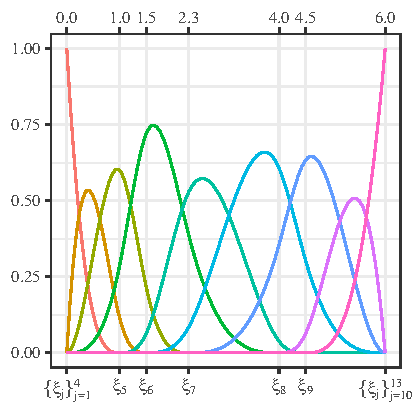
\includegraphics[width=\linewidth]{figures/a}
  \caption{\label{fig:graphic_a}}
  \end{subfigure}
  ~
  \begin{subfigure}[t]{0.48\linewidth}
  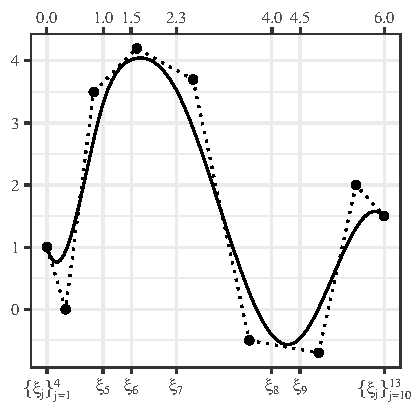
\includegraphics[width=\linewidth]{figures/b}
  \caption{\label{fig:graphic_b}}
  \end{subfigure}
  \caption[Short Caption for List of Figures]{Long Caption with lots of details
  \ldots \label{fig:graphic}}
\end{figure}

\lipsum

\section{Discussion}
\lipsum[4]


\chapter{\uppercase{Second Publishable Paper} \label{chapter:03}}

\section{Summary}
Abstract from second publishable paper.

\section{Intro}

Hey, remember in Chapter~\ref{chapter:02} when I said you'll have to repeat
yourself?  Well, \eqref{eq:chap2_example_eq} and \eqref{eq:chap3_example_eq}
should look the same, but have different \LaTeX\ labels an be referenced
correctly.

\begin{equation}
\label{eq:chap3_example_eq}
  \omega_{jk}\left(x\right) =
  \begin{cases}
  \hfil 0                                        & \hfil x \leq \xi_{j} \\
  \frac{x - \xi_{j}} {\xi_{j + k - 1} - \xi_{j}} & \xi_{j} < x < \xi_{j+ k - 1} \\
  \hfil 1                                        & \hfil \xi_{j + k - 1} \leq x
  \end{cases}.
\end{equation}

\section{Details}
\lipsum
 
\begin{figure}
\centering
  \begin{subfigure}[t]{0.48\linewidth}
  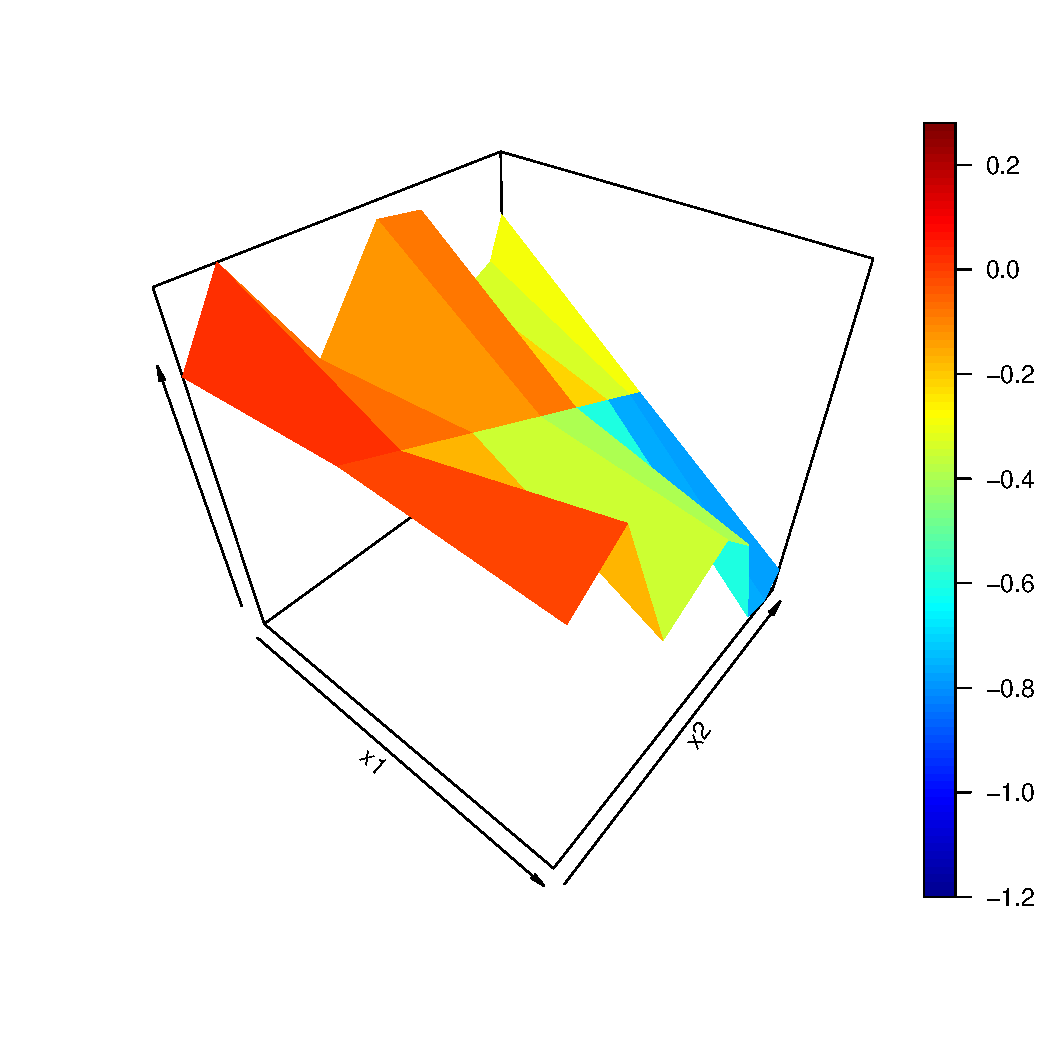
\includegraphics[width=\linewidth]{figures/c}
  \caption{\label{fig:graphic_c}}
  \end{subfigure}
  ~
  \begin{subfigure}[t]{0.48\linewidth}
  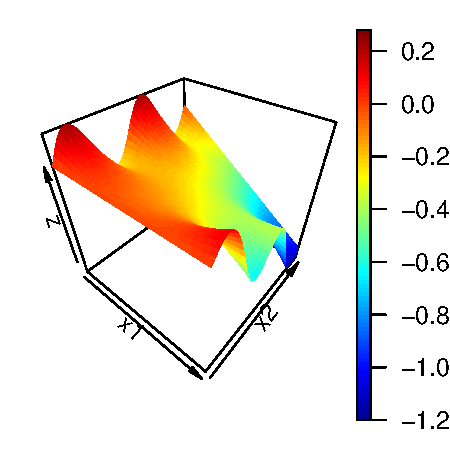
\includegraphics[width=\linewidth]{figures/d}
  \caption{\label{fig:graphic_d}}
  \end{subfigure}
  \caption[Another short caption for List of Figures]{Long Caption with lots of details
  \ldots \label{fig:chap3_graphic}}
\end{figure}

\section{Discussion}
\lipsum



\chapter{\uppercase{Third Publishable Paper} \label{chapter:04}}

\section{Summary}
You can do this\ldots

\section{Details}
\lipsum[1]

\subsection{Details Part 1}
\lipsum

\subsection{Details Part 2}
\lipsum

\section{Discussion}
\lipsum

\chapter{\uppercase{Discussion} \label{chapter:05}}

\section{Summary of Dissertation}
\lipsum

\section{Continuing Work}
\lipsum


% ---------------------------------------------------------------------------- %
\renewcommand\bibname{REFERENCES}
\singlespacing

\nocite{*}
\bibliographystyle{ucdDissertation}
\bibliography{references,r-references}

\doublespacing

% ---------------------------------------------------------------------------- %
% had to do some TOC shenanigans, so please use the ucdappendix command instead
% of regular old \appendix
\ucdappendix

\chapter{\uppercase{Abbreviations and Notation} \label{appendix-notation}}

\section{Abbreviations}

\begin{description}[leftmargin=!,labelwidth=0.5in,font=\normalfont]
  \item[CNR]  Control net reduction.
  \item[CPR]  Control polygon reduction.
  \item[CRAN] The Comprehensive \proglang{R} Archive Network.
  \item[DHS]  Daily Hormone Study, a sub-study of SWAN.
  \item[DLT]  Day of Luteal Transition.
  \item[PDG]  Prognanediol-glucuronid, is the urine metabolite of progesterone.
  \item[SWAN] The Study of Women's Health Across the Nation.  
  \item[TTM]  Time-to-menopause
\end{description}

\section{Mathematic Notation}

\subsection{General Notation}

\begin{description}[leftmargin=!, labelwidth=0.7in]
  \item[$x$]             italicized, Roman or Greek letter, denotes a scalar values 
  \item[$\bs{x}$]        italicized, bold, lowercase Roman or Greek letter, denotes a column vector or set.
  \item[$\bs{X}$]        italicized, bold, uppercase Roman or Greek letter, denotes a matrix or set.
  \item[$\card{\bs{x}}$] cardinality, number of elements, of the vector or set $\bs{x}$ 
  \item[$x \in (a, b)$]  the value $x$ is within the interval such that $a < x < b$
  \item[{$x \in (a, b]$}]  the value $x$ is within the interval such that $a < x \leq b$
  \item[$x \in [a, b)$]  the value $x$ is within the interval such that $a \leq x < b$
  \item[{$x \in [a, b]$}]  the value $x$ is within the interval such that $a \leq x \leq b$ 
  \item[$1_{A}\left(x\right)$] the indicator function,\[1_{A}\left(x \right) = \begin{cases} 1 & x \in A \\ 0 & x \notin A \end{cases}.\] 
  \item[$\bs{1}_n$] an column vector of $n$ $1$s
  \item[$\bs{I}$] the identity matrix
  \item[$\bs{I}_n$] the $n \times n$ identity matrix
  \item[$\bs{X}^{-1}$] the inverse matrix, that is, $\bs{X}^{-1} \bs{X} = \bs{I}.$
  \item[$\bs{X}^{T}$] transpose
  \item[$\otimes$] Kronecker product
  \item[$\odot$] element-wise multiplication
\end{description}

\subsection{Sets}

\begin{description}[leftmargin=!, labelwidth=0.8in]
  \item[$\{x, y, z, \ldots\}$]  The set comprising the elements of $x,$ $y,$ $z,$ $\ldots$ 
  \item[$\{x, y, z\} \backslash x$]  The set comprising the elements of $y$ and $z,$ that is, the backslash removes elements from the set.
  \item[$\left\{x_i\right\}_{i = 1}^{n}$]  The set comprising the elements of $x_1, x_2, x_3, \ldots, x_n.$ 
  \item[$\mathbb{R}$] Set of real numbers 
  \item[$\bs{x} \in \mathbb{R}^n$] $\bs{x}$ is a vector with $n$ elements, all of which are real numbers.
\end{description}

\subsection{Statistical Distributions}
\begin{description}[leftmargin=!, labelwidth=0.8in]
  \item[$\mathcal{N} \left( \mu, \sigma^2 \right)$] the uni-variable Gaussian distribution with mean $\mu$ and variance $\sigma^2.$ 
  \item[$\mathcal{N} \left( \bs{\mu}, \bs{\Sigma} \right)$] the multi-variable Gaussian distribution with mean vector $\bs{\mu}$ and variance-covariance matrix $\bs{\Sigma}.$
  \item[$\phi(x)$] The standard Gaussian density function.
\end{description}

% ---------------------------------------------------------------------------- %
% additional appendices
\chapter{\uppercase{Appendix Header}}

\lipsum[5]


% ---------------------------------------------------------------------------- %
\end{document}
% ---------------------------------------------------------------------------- %
